% UniPlan final report, ENGG2112 2026 S2.
% Built from the unit's 2026 report template (Final Report Template.zip, 23 Sep 2026),
% adapted for XeTeX: compile with `tectonic -X compile main.tex` from this folder.
% Every number in the text comes from generated/numbers.tex (report/scripts/make_numbers.py).
\documentclass[12pt,a4paper]{article}

\usepackage{graphicx}
\usepackage[top=1in, bottom=1in, left=1in, right=1in]{geometry}
\usepackage{amsmath,amssymb}
\usepackage{booktabs,array}
\usepackage{xcolor}
\usepackage{tikz}
\usetikzlibrary{positioning,arrows.meta,fit}
\usepackage[font=small,labelfont=bf,skip=4pt]{caption}
\usepackage{enumitem}
\setlist{nolistsep,noitemsep}
\usepackage{cite}
% Chinese for the original prompts in Appendix A (macOS system font; the font file is not redistributed).
\usepackage{xeCJK}
\setCJKmainfont[Path=/System/Library/Fonts/,FontIndex=0]{Hiragino Sans GB.ttc}
\xeCJKsetup{CJKspace=true}
\usepackage[hidelinks]{hyperref}

\linespread{1.06}
\setlength{\parskip}{8pt plus2pt minus2pt}
\widowpenalty 10000
\clubpenalty 10000

\definecolor{accent}{HTML}{5B4E9E}
\newcommand{\HRule}{\rule{\linewidth}{0.5mm}}
\newcommand{\repo}{\textit{[public repository link to be added]}}

% Generated by report/scripts/make_numbers.py from the raw result files. Do not edit by hand.
% All test sentences, personas, labels and exams are synthetic (AI-written); no real students.
% data/processed/*.csv: distinct unit_code over all snapshot CSVs
\newcommand{\dUnits}{7}
% data/processed/*.csv: distinct meeting_id
\newcommand{\dMeetings}{1{,}240}
% data/processed/*.csv: distinct option_id
\newcommand{\dOptions}{242}
% data/processed/*.csv: distinct group_id
\newcommand{\dGroups}{25}
% data/locations/buildings.json: len(buildings)
\newcommand{\dBuildings}{19}
% report/data/timetable_counts.json (report/scripts/count_timetables.py): ENGG2112+AMME2301 feasible_count
\newcommand{\ttTwo}{6{,}800}
% report/data/timetable_counts.json (report/scripts/count_timetables.py): ENGG2112+AMME2301 distinct_GDO
\newcommand{\ttTwoDistinct}{172}
% report/data/timetable_counts.json (report/scripts/count_timetables.py): ENGG2112+AMME2301 non_dominated
\newcommand{\ttTwoFront}{4}
% report/data/timetable_counts.json (report/scripts/count_timetables.py): five units feasible_count
\newcommand{\ttFive}{24{,}304{,}704}
% report/data/timetable_counts.json (report/scripts/count_timetables.py): five units non_dominated
\newcommand{\ttFiveFront}{2}
% report/data/timetable_counts.json (report/scripts/count_timetables.py): five units seconds_full_flow (Mac), 1 decimal
\newcommand{\ttFiveSec}{3.4}
% llm/parse/output/synthetic_clauses.jsonl: rows (= synthetic_meta.json kept)
\newcommand{\sClauses}{1{,}781}
% llm/parse/output/synthetic_clauses.jsonl: rows with language == zh
\newcommand{\sZh}{642}
% llm/parse/output/synthetic_clauses.jsonl: rows with language == mix
\newcommand{\sMix}{543}
% llm/parse/output/synthetic_clauses.jsonl: rows with language == en
\newcommand{\sEn}{596}
% llm/parse/output/train_round2.jsonl: rows with split == train
\newcommand{\sTrainTwo}{1{,}757}
% llm/parse/output/train_round2.jsonl: rows with split == val
\newcommand{\sValTwo}{278}
% llm/parse/data/train_claude.csv: rows (one per clause)
\newcommand{\sHardOne}{141}
% llm/parse/data/train_claude_round2.csv: rows (one per clause)
\newcommand{\sHardTwo}{201}
% train_claude.csv + train_claude_round2.csv rows (Claude-written hard clauses)
\newcommand{\sHardAll}{342}
% llm/parse/output/review_round1_claude.jsonl: rows (= review_round1_stats.json grading.graded)
\newcommand{\sGraded}{476}
% llm/parse/data/test_claude.csv: rows with a sentence_id (one per sentence)
\newcommand{\sTestOneS}{142}
% llm/parse/data/test_claude.csv: rows (one per clause)
\newcommand{\sTestOneC}{174}
% llm/parse/data/test_claude_v2.csv: rows with a sentence_id (one per sentence)
\newcommand{\sTestTwoS}{126}
% llm/parse/data/test_claude_v2.csv: rows (one per clause)
\newcommand{\sTestTwoC}{146}
% llm/parse/exam/exam.csv: rows with a sentence_id (one per sentence)
\newcommand{\sExamS}{304}
% llm/parse/exam/exam.csv: rows (one per clause)
\newcommand{\sExamC}{461}
% llm/rank/data/personas.json: len(personas)
\newcommand{\sPersonas}{140}
% llm/rank/data/personas.json: personas with split == train
\newcommand{\sTrainPersonas}{120}
% llm/rank/data/personas.json: personas with split == test
\newcommand{\sTestPersonas}{20}
% llm/rank/output/labels_v3d_qwen2.5_14b.jsonl: rows
\newcommand{\sLabels}{2{,}471}
% llm/rank/output/labels_v3d_qwen2.5_14b_corrected.jsonl: rows with corrected_by == claude
\newcommand{\sReplaced}{17}
% llm/rank/exam/personas.json: len(personas)
\newcommand{\sRankExamPersonas}{20}
% llm/rank/exam/questions.jsonl: rows
\newcommand{\sRankQ}{540}
% llm/rank/exam/answers.jsonl: choice red or blue (scored pairs)
\newcommand{\sRankScored}{485}
% llm/rank/exam/answers.jsonl: choice 'about the same' (not scored)
\newcommand{\sRankSame}{55}
% llm/rank/output/labels_v3d_qwen2.5_14b.jsonl: source == model rows with label A or B, 1853/2061
\newcommand{\tConsistent}{89.9}
% llm/rank/output/labels_v3d_qwen2.5_14b.jsonl: mean seconds over the 2061 asked pairs (= 4.4485; the summary JSON rounds it to 4.45)
\newcommand{\tSec}{4.4}
% check_answers_claude.jsonl + check_pairs_key.json (teacher_audit) vs labels_v3d_qwen2.5_14b.jsonl (source == model): 156/173
\newcommand{\tClaudeAgree}{90.2}
% same: audited 14B-asked pairs where both gave a side
\newcommand{\tClaudeN}{173}
% llm/rank/output/labels_v3d_qwen2.5_14b.jsonl: rows with source == model
\newcommand{\tAsked}{2{,}061}
% same: source == model rows whose two orders agree (label A or B)
\newcommand{\tKept}{1{,}853}
% same: rows decided by code (source != model)
\newcommand{\tCode}{410}
% report/data/rank_exam_paired.json difference (trained LR minus equal weights), points
\newcommand{\rDiffEq}{5.2}
% report/data/rank_exam_paired.json difference_ci95[0] (paired bootstrap over personas, 10,000 reps, seed 2112)
\newcommand{\rDiffEqLo}{\ensuremath{-}4.6}
% report/data/rank_exam_paired.json difference_ci95[1]
\newcommand{\rDiffEqHi}{14.7}
% summary only: llm/parse/exam/PROVENANCE.md, regex 'dropped N candidate sentences'
\newcommand{\sExamDropped}{93}
% report/data/timetable_counts.json ENGG2112+AMME2301 search.full_options
\newcommand{\ttTwoFull}{29}
% report/data/timetable_counts.json ENGG2112+AMME2301 search.total_options
\newcommand{\ttTwoOptions}{71}
% llm/rank/output/rank_pilot.json summary.pairs (= v3d 14B pairs)
\newcommand{\tPilotN}{30}
% llm/rank/output/rank_pilot.json summary.consistent (prompt v1, qwen2.5:7b)
\newcommand{\tPilotFirst}{16}
% llm/rank/output/rank_pilot_v3d_qwen2.5_14b_summary.json asked_model (pairs put to the model)
\newcommand{\tPilotAsked}{22}
% same: consistent_all minus the code-decided pairs; matches consistent_rate_asked
\newcommand{\tPilotAskedOK}{20}
% llm/rank/output/rank_pilot_v3d_qwen2.5_14b_summary.json consistent_all (prompt v3d, qwen2.5:14b, incl. code-decided pairs)
\newcommand{\tPilotFinal}{28}
% llm/rank/output/exam_report.json llm_seconds_per_call (qwen2.5:14b on the exam)
\newcommand{\rQwenSec}{2.1}
% llm/rank/data/personas.json: split == train and round == 1 (model.json is the round-1 fit)
\newcommand{\rDeployPersonas}{60}
% llm/rank/output/labels_v3d_qwen2.5_14b_corrected.jsonl: round-1 training personas, label A or B
\newcommand{\rDeployTeacher}{836}
% llm/rank/output/model_comparison.json train_pairs minus the teacher pairs (free code-decided pairs)
\newcommand{\rDeployCode}{1{,}351}
% llm/rank/output/model_comparison.json: LR with student terms, pairwise_accuracy on the 20 held-out personas (teacher labels)
\newcommand{\rHeldOne}{90.5}
% llm/rank/output/model_comparison_round2.json: same model refitted on 120 personas (not shipped)
\newcommand{\rHeldTwo}{90.0}
% llm/rank/output/model_comparison.json: code-decided dominance pairs / train_pairs (deployed model)
\newcommand{\rDomShare}{61.8}
% llm/rank/output/model_comparison.json: 成对逻辑回归 + 学生交叉项 accuracy_by_label_source.model (held-out pairs Qwen 14B judged)
\newcommand{\rHeldTeacherLR}{87.0}
% llm/rank/output/model_comparison.json: 等权打分 accuracy_by_label_source.model (held-out pairs Qwen 14B judged)
\newcommand{\rHeldTeacherEq}{65.7}
% llm/rank/exam/llm_qwen2.5_14b.jsonl: pairs where 14B chose the timetable shown first (red), 317/540
\newcommand{\rQwenFirst}{58.7}
% llm/parse/output/train_round2.jsonl: split == train and source claude_*
\newcommand{\sClaudeTrain}{315}
% same: 315/1757
\newcommand{\sClaudeTrainPct}{17.9}
% llm/parse/output/exam/parse_results.json: model == linear-r1, val.accuracy
\newcommand{\pLinVal}{88.8}
% llm/parse/output/exam/parse_results.json: model == keywords, val.accuracy
\newcommand{\pKeyVal}{71.2}
% output/pipeline/…_exam.json: status_gold == no_feasible, 110/304 (same 110 as plNoFit)
\newcommand{\plNoFitPct}{36.2}
% output/pipeline/…_exam.json: median total_seconds over 196 sentences with status_parsed == ready
\newcommand{\plMedianRec}{0.61}
% llm/parse/output/lora_train_log_7b_r2.json: settings.rank
\newcommand{\loraRank}{16}
% llm/parse/windows/train_lora.py: lora_alpha = 2 * rank (rank from llm/parse/output/lora_train_log_7b_r2.json)
\newcommand{\loraAlpha}{32}
% llm/parse/output/lora_train_log_7b_r2.json: settings.epochs
\newcommand{\loraEpochs}{3}
% llm/parse/output/lora_train_log_7b_r2.json: settings.lr = 0.0002
\newcommand{\loraLR}{\ensuremath{2\times10^{-4}}}
% llm/parse/output/lora_train_log_7b_r2.json: training_minutes (round 2)
\newcommand{\loraMinutes}{13.4}
% llm/parse/output/lora_train_log_7b.json: training_minutes (round 1)
\newcommand{\loraMinutesOne}{10.4}
% llm/parse/output/lora_train_log_7b_r2.json: best_epoch (round 2)
\newcommand{\loraBest}{3}
% llm/parse/output/exam/parse_results.json: model == "keywords", test.accuracy = 391/461
\newcommand{\pKeyC}{84.8}
% llm/parse/output/exam/parse_results.json: model == "keywords", test.sentence_all_right = 216/304
\newcommand{\pKeyS}{71.1}
% llm/parse/output/exam/parse_results.json: model == "linear-r1", test.accuracy = 390/461
\newcommand{\pLinC}{84.6}
% llm/parse/output/exam/parse_results.json: model == "linear-r1", test.sentence_all_right = 205/304
\newcommand{\pLinS}{67.4}
% llm/parse/output/exam/parse_results.json: model == "ollama-v2:qwen2.5:7b", test.accuracy = 397/461
\newcommand{\pZeroC}{86.1}
% llm/parse/output/exam/parse_results.json: model == "ollama-v2:qwen2.5:7b", test.sentence_all_right = 211/304
\newcommand{\pZeroS}{69.4}
% llm/parse/output/exam/parse_results.json: model == "ollama-short:uniplan-parse-7b", test.accuracy = 426/461
\newcommand{\pRoneC}{92.4}
% llm/parse/output/exam/parse_results.json: model == "ollama-short:uniplan-parse-7b", test.sentence_all_right = 231/304
\newcommand{\pRoneS}{76.0}
% llm/parse/output/exam/parse_results.json: model == "ollama-short:uniplan-parse-7b-r2", test.accuracy = 437/461
\newcommand{\pRtwoC}{94.8}
% llm/parse/output/exam/parse_results.json: model == "ollama-short:uniplan-parse-7b-r2", test.sentence_all_right = 237/304
\newcommand{\pRtwoS}{78.0}
% 95% bootstrap (sentences resampled, 10,000 reps, seed 2112) recomputed with report/scripts/parse_exam_ci.py; matches report/data/parse_exam_ci.json methods."Qwen 7B QLoRA round 2".clause_ci[0] (unrounded 0.926606)
\newcommand{\pRtwoCLo}{92.7}
% 95% bootstrap (sentences resampled, 10,000 reps, seed 2112) recomputed with report/scripts/parse_exam_ci.py; matches report/data/parse_exam_ci.json methods."Qwen 7B QLoRA round 2".clause_ci[1] (unrounded 0.967462)
\newcommand{\pRtwoCHi}{96.7}
% 95% bootstrap (sentences resampled, 10,000 reps, seed 2112) recomputed with report/scripts/parse_exam_ci.py; matches report/data/parse_exam_ci.json methods."Qwen 7B QLoRA round 2".sentence_ci[0] (unrounded 0.733553)
\newcommand{\pRtwoSLo}{73.4}
% 95% bootstrap (sentences resampled, 10,000 reps, seed 2112) recomputed with report/scripts/parse_exam_ci.py; matches report/data/parse_exam_ci.json methods."Qwen 7B QLoRA round 2".sentence_ci[1] (unrounded 0.825658)
\newcommand{\pRtwoSHi}{82.6}
% llm/parse/output/exam/parse_results.json: round 2 minus pRoneC (clauses), exact counts
\newcommand{\pDiffOneC}{2.4}
% paired bootstrap recomputed as in report/scripts/parse_exam_ci.py; report/data/parse_exam_ci.json differences."Qwen 7B QLoRA round 2 minus Qwen 7B QLoRA round 1".clause_ci[0] (unrounded 0.002217)
\newcommand{\pDiffOneCLo}{0.2}
% paired bootstrap recomputed as in report/scripts/parse_exam_ci.py; report/data/parse_exam_ci.json differences."Qwen 7B QLoRA round 2 minus Qwen 7B QLoRA round 1".clause_ci[1] (unrounded 0.044543)
\newcommand{\pDiffOneCHi}{4.5}
% llm/parse/output/exam/parse_results.json: round 2 minus pRoneS (whole sentences), exact counts
\newcommand{\pDiffOneS}{2.0}
% paired bootstrap recomputed as in report/scripts/parse_exam_ci.py; report/data/parse_exam_ci.json differences."Qwen 7B QLoRA round 2 minus Qwen 7B QLoRA round 1".sentence_ci[0] (unrounded -0.013158)
\newcommand{\pDiffOneSLo}{\ensuremath{-}1.3}
% paired bootstrap recomputed as in report/scripts/parse_exam_ci.py; report/data/parse_exam_ci.json differences."Qwen 7B QLoRA round 2 minus Qwen 7B QLoRA round 1".sentence_ci[1] (unrounded 0.052632)
\newcommand{\pDiffOneSHi}{5.3}
% llm/parse/output/exam/parse_results.json: round 2 minus pZeroC (clauses), exact counts
\newcommand{\pDiffZeroC}{8.7}
% paired bootstrap recomputed as in report/scripts/parse_exam_ci.py; report/data/parse_exam_ci.json differences."Qwen 7B QLoRA round 2 minus Qwen 7B zero-shot, prompt v2".clause_ci[0] (unrounded 0.057495)
\newcommand{\pDiffZeroCLo}{5.7}
% paired bootstrap recomputed as in report/scripts/parse_exam_ci.py; report/data/parse_exam_ci.json differences."Qwen 7B QLoRA round 2 minus Qwen 7B zero-shot, prompt v2".clause_ci[1] (unrounded 0.117021)
\newcommand{\pDiffZeroCHi}{11.7}
% llm/parse/output/exam/parse_results.json: round 2 minus pZeroS (whole sentences), exact counts
\newcommand{\pDiffZeroS}{8.6}
% paired bootstrap recomputed as in report/scripts/parse_exam_ci.py; report/data/parse_exam_ci.json differences."Qwen 7B QLoRA round 2 minus Qwen 7B zero-shot, prompt v2".sentence_ci[0] (unrounded 0.046053)
\newcommand{\pDiffZeroSLo}{4.6}
% paired bootstrap recomputed as in report/scripts/parse_exam_ci.py; report/data/parse_exam_ci.json differences."Qwen 7B QLoRA round 2 minus Qwen 7B zero-shot, prompt v2".sentence_ci[1] (unrounded 0.128289)
\newcommand{\pDiffZeroSHi}{12.8}
% llm/parse/output/exam/parse_results.json: round 2 minus pKeyC (clauses), exact counts
\newcommand{\pDiffKeyC}{10.0}
% paired bootstrap recomputed as in report/scripts/parse_exam_ci.py; report/data/parse_exam_ci.json differences."Qwen 7B QLoRA round 2 minus keyword rules".clause_ci[0] (unrounded 0.062099)
\newcommand{\pDiffKeyCLo}{6.2}
% paired bootstrap recomputed as in report/scripts/parse_exam_ci.py; report/data/parse_exam_ci.json differences."Qwen 7B QLoRA round 2 minus keyword rules".clause_ci[1] (unrounded 0.138393)
\newcommand{\pDiffKeyCHi}{13.8}
% llm/parse/output/exam/parse_results.json: round 2 minus pKeyS (whole sentences), exact counts
\newcommand{\pDiffKeyS}{6.9}
% paired bootstrap recomputed as in report/scripts/parse_exam_ci.py; report/data/parse_exam_ci.json differences."Qwen 7B QLoRA round 2 minus keyword rules".sentence_ci[0] (unrounded 0.023026)
\newcommand{\pDiffKeySLo}{2.3}
% paired bootstrap recomputed as in report/scripts/parse_exam_ci.py; report/data/parse_exam_ci.json differences."Qwen 7B QLoRA round 2 minus keyword rules".sentence_ci[1] (unrounded 0.115132)
\newcommand{\pDiffKeySHi}{11.5}
% llm/parse/output/exam/parse_results.json: test.split_right (same for every method)
\newcommand{\pSplit}{76.3}
% llm/parse/output/exam/clarify_results.json: exam."model run time".clauses.asked / clauses = 77/461
\newcommand{\cAsked}{16.7}
% llm/parse/output/exam/clarify_results.json: exam."model run time".clauses.wrong
\newcommand{\cWrong}{24}
% llm/parse/output/exam/clarify_results.json: exam."model run time".clauses.asked
\newcommand{\cAskedN}{77}
% llm/parse/output/exam/clarify_results.json: exam."model run time".sentences.sentences_with_a_question (a clarifying question or an offer)
\newcommand{\cSentWithQ}{49.0}
% llm/parse/output/exam/clarify_results.json: exam."model run time".clauses.caught_share * wrong
\newcommand{\cCovered}{21}
% llm/parse/output/exam/clarify_results.json: exam."model run time".clauses.caught_share = 21/24
\newcommand{\cCoveredPct}{87.5}
% llm/parse/output/exam/clarify_results.json: exam."model run time".clauses.fixable_share * wrong (right answer among the offered options)
\newcommand{\cOption}{18}
% llm/parse/output/exam/clarify_results.json: exam."model run time": (clauses - wrong + offered fixes) / clauses = 455/461 (projection: assumes students pick the right option)
\newcommand{\cProjected}{98.7}
% llm/parse/output/exam/clarify_results.json: exam."model run time".sentences.questions_per_sentence
\newcommand{\cPerSentence}{0.61}
% llm/rank/output/exam_report.json: results[trained LR (model.json)].pairwise_accuracy = 404/485
\newcommand{\rLR}{83.3}
% llm/rank/output/exam_report.json: results[trained LR (model.json)].ci95[0] (bootstrap over personas, 2,000 reps)
\newcommand{\rLRLo}{75.6}
% llm/rank/output/exam_report.json: results[trained LR (model.json)].ci95[1]
\newcommand{\rLRHi}{90.2}
% llm/rank/output/exam_report.json: results[trained LR (model.json)].top3_hit
\newcommand{\rLRTop}{0.79}
% llm/rank/output/exam_report.json: results[equal weights].pairwise_accuracy = 379/485
\newcommand{\rEq}{78.1}
% llm/rank/output/exam_report.json: results[equal weights].ci95[0] (bootstrap over personas, 2,000 reps)
\newcommand{\rEqLo}{72.8}
% llm/rank/output/exam_report.json: results[equal weights].ci95[1]
\newcommand{\rEqHi}{83.2}
% llm/rank/output/exam_report.json: results[equal weights].top3_hit
\newcommand{\rEqTop}{0.68}
% llm/rank/output/exam_report.json: results[cares-only rule].pairwise_accuracy = 346/485
\newcommand{\rCares}{71.3}
% llm/rank/output/exam_report.json: results[cares-only rule].top3_hit
\newcommand{\rCaresTop}{0.53}
% llm/rank/output/exam_report.json: results[Qwen 14B each pair].pairwise_accuracy = 318/485
\newcommand{\rQwen}{65.6}
% llm/rank/output/exam_report.json: results[Qwen 14B each pair].ci95[0] (bootstrap over personas, 2,000 reps)
\newcommand{\rQwenLo}{59.3}
% llm/rank/output/exam_report.json: results[Qwen 14B each pair].ci95[1]
\newcommand{\rQwenHi}{71.9}
% llm/rank/output/exam_report.json: results[Qwen 14B picks top 3].top3_hit
\newcommand{\rQwenTop}{0.59}
% llm/rank/output/exam_report.json: random_baseline.top3_hit
\newcommand{\rRandTop}{0.38}
% llm/rank/output/exam_report.json: top3_ceiling
\newcommand{\rCeiling}{0.93}
% llm/rank/output/exam_report.json: results[trained LR].best_in_top3, as a percentage
\newcommand{\rFirstInTop}{96.7}
% llm/rank/exam/answers_second.jsonl vs answers.jsonl: same side where both picked a side, 112/136
\newcommand{\rAgree}{82.4}
% llm/rank/exam/answers_second.jsonl vs answers.jsonl: same side
\newcommand{\rAgreeHit}{112}
% llm/rank/exam/answers_second.jsonl vs answers.jsonl: pairs where both picked a side
\newcommand{\rAgreeOf}{136}
% llm/rank/exam/answers_second.jsonl vs answers.jsonl: distinct persona_id (via questions.jsonl)
\newcommand{\rAgreePersonas}{6}
% llm/rank/output/ablation_round1.json: accuracy(full) - accuracy(student terms dropped), in points
\newcommand{\rAblInteraction}{15.0}
% llm/rank/output/ablation_round1.json: accuracy(full) - accuracy(three main features dropped), in points
\newcommand{\rAblMain}{5.0}
% llm/rank/output/learning_curve.json: curve.with_program_pairs (sample random), personas 60: accuracy.mean over 5 draws
\newcommand{\rCurveSixty}{89.6}
% llm/rank/output/learning_curve.json: curve.with_program_pairs (sample random), personas 120: accuracy.mean
\newcommand{\rCurveMax}{89.7}
% summary only: llm/rank/output/RESULTS.md:148 (rank() on 20 real candidates incl. features), regex
\newcommand{\rMs}{3.6}
% output/pipeline/pipeline_eval_uniplan-parse-7b-r2_model_exam.json: records with exact == true
\newcommand{\plExactN}{237}
% output/pipeline/pipeline_eval_uniplan-parse-7b-r2_model_exam.json: 237/304 records exact
\newcommand{\plExact}{78.0}
% output/pipeline/pipeline_eval_uniplan-parse-7b-r2_model_exam.json: records with status_parsed == ready
\newcommand{\plPlannable}{196}
% output/pipeline/pipeline_eval_uniplan-parse-7b-r2_model_exam.json: plannable records where any pick has violations (uniplan.advisor.hard_violations)
\newcommand{\plViol}{16}
% output/pipeline/pipeline_eval_uniplan-parse-7b-r2_model_exam.json: 16/196
\newcommand{\plViolPct}{8.2}
% output/pipeline/pipeline_eval_uniplan-parse-7b-r2_model_exam.json: picks_parsed[0] == picks_gold[0]
\newcommand{\plSameFirstN}{174}
% output/pipeline/pipeline_eval_uniplan-parse-7b-r2_model_exam.json: records with both picks_parsed and picks_gold
\newcommand{\plSameFirstOf}{188}
% output/pipeline/pipeline_eval_uniplan-parse-7b-r2_model_exam.json: 174/188
\newcommand{\plSameFirst}{92.6}
% output/pipeline/pipeline_eval_uniplan-parse-7b-r2_model_exam.json: median total_seconds (sentence to recommendation)
\newcommand{\plMedian}{0.58}
% output/pipeline/pipeline_eval_uniplan-parse-7b-r2_model_exam.json: max total_seconds
\newcommand{\plMax}{1.42}
% output/pipeline/nearest_eval_exam.json: records with strict == no_feasible (all got closest timetables)
\newcommand{\plNoFit}{110}
% output/pipeline/nearest_eval_exam.json: mean picks[0].limits_broken over those records
\newcommand{\plNoFitBreaks}{1.18}
% output/explain/explain_eval_template_en_exam.json: picks with template_passes
\newcommand{\exTemplatePass}{571}
% output/explain/explain_eval_template_en_exam.json: picks over records with status == ready
\newcommand{\exPicks}{571}
% output/explain/explain_eval_template_en_exam.json: template_feature == main_feature (pick 1)
\newcommand{\exMainN}{185}
% output/explain/explain_eval_template_en_exam.json: ready records with a main_feature
\newcommand{\exMainOf}{192}
% output/explain/explain_eval_template_en_exam.json: 185/192 (same in output/explain/explain_eval_qwen2.5-7b_en_exam.json)
\newcommand{\exMain}{96.4}
% output/explain/explain_eval_qwen2.5-7b_en_exam.json: picks with model_passed
\newcommand{\exRewritePass}{194}
% output/explain/explain_eval_qwen2.5-7b_en_exam.json: picks with a model_text
\newcommand{\exRewriteOf}{570}
% output/explain/explain_eval_qwen2.5-7b_en_exam.json: 194/570
\newcommand{\exRewrite}{34.0}
% summary only: output/explain/README.md:84-86 (manual check by Claude), regex
\newcommand{\exManualWrong}{10}
% summary only: output/explain/README.md:84 (manual check by Claude), regex
\newcommand{\exManualOf}{30}
% report/data/pareto_example.json: example.units (e187)
\newcommand{\figUnits}{3}
% report/data/pareto_example.json: example.conditions.max_daily_span / 60
\newcommand{\figSpan}{7}
% report/data/pareto_example.json: example.feasible_count
\newcommand{\figFeasible}{5{,}072}
% report/data/pareto_example.json: example.profiles (distinct G/D/O)
\newcommand{\figTypes}{55}
% report/data/pareto_example.json: len(example.front)
\newcommand{\figFront}{3}
% report/data/pareto_example.json: exam sentences whose intended conditions allow a timetable
\newcommand{\figStudents}{194}
% report/data/pareto_example.json: students with front <= 4
\newcommand{\figSmallFront}{190}


\begin{document}

%===========================================================
\begin{titlepage}
	\begin{center}
		
\includegraphics[width=0.55\textwidth]{figures/usyd-logo.png}~\\[2cm]
		\HRule \\[0.4cm]
		{ \LARGE
			\textbf{Project Report for ENGG2112}\\[0.4cm]
			\emph{UniPlan: From a Student's Sentence to\\Three Clash-Free Timetables}\\[0.4cm]
		}
		\HRule \\[1.5cm]
		{ \large
			% The author line with the student ID lives in author.tex, which is not committed.
			\InputIfFileExists{author}{}{Han Dongrui, Mechanical Engineering} \\[0.1cm]
		}
		\vfill
		Code: \repo \\[0.8cm]
		\textsc{\large Faculty of Engineering}\\[0.4cm]
		{\large 1 November 2026}
	\end{center}
\end{titlepage}

\pagenumbering{roman}
\begin{center}
	\subsection*{Executive Summary}
\end{center}

\noindent Students who work, commute or care for family must fit their classes around fixed commitments, and building a timetable by hand from thousands of valid combinations is slow. UniPlan lets a student describe their week in one sentence and returns three clash-free timetables with a reason for each.

The system follows an engineering pattern: learned models interpret and rank, and verifiable code decides what is allowed. Rules split the sentence into clauses, a Qwen2.5-7B model fine-tuned with QLoRA on a laptop GPU labels each one, and rules read the days, times and amounts; the student confirms the result or answers a short clarifying question. A deterministic scheduler then finds every valid timetable exactly, so a clash is never recommended. A logistic regression with student-specific weights ranks the candidates, and its per-feature contributions become the reasons.

There was no real student data and no participants were recruited, so every sentence, persona, label and test was written by AI models: Qwen generated most of the training data, and fresh Claude agents wrote and answered the final exams. On the final exams, which were committed after the models were frozen and scored once, the parser read \pRtwoC\% of clauses and \pRtwoS\% of whole sentences correctly (keyword rules: \pKeyC\% and \pKeyS\%), and its clarifying questions covered \cCoveredPct\% of its remaining errors. The ranker agreed with independent answers on \rLR\% of timetable pairs, level with equal weights (\rEq\%) within the exam's uncertainty and well ahead of asking Qwen2.5-14B once per pair (\rQwen\%). End to end, a sentence for two to four units becomes three recommendations in a median of \plMedianRec{}~s. The trained ranker scored higher than equal weights, but the paired interval included zero, so its advantage is unproven.

These results show that the method works on AI-written students, not that it helps real ones. Before wider use we recommend a pilot with real students, accuracy checks for students who write in a second language, and care with demand concentration and the privacy of what students write. The same structure could serve engineering scheduling problems such as production planning and crew rostering.

\newpage

\setcounter{tocdepth}{1}
\tableofcontents
\addtocontents{toc}{\protect\thispagestyle{empty}}
\newpage
\pagenumbering{arabic}

\section{Background and Motivation}\label{sec:intro}

Every semester, University of Sydney students build their own timetable from the classes the university publishes~\cite{usyd_timetable}, choosing one class from every activity group so that nothing clashes. The combinations multiply quickly: ENGG2112 and AMME2301 alone allow \ttTwo{} clash-free timetables in Semester~2, 2026, even with full classes excluded, and five engineering units allow \ttFive{}.

For students who work, commute or care for family, the choice decides whether study fits around the rest of their life. In its 2017 Student Finances Survey, Universities Australia reported that more than four in five students were in paid work, 30\% of full-time students worked more than 20 hours a week, and more than a quarter of full-time students regularly missed classes because of work~\cite{ua_finances_2017}. These students state their requirements in words (``I work Tuesday and Thursday nights, and mornings aren't great''), not as weights or blocked grid cells.

Seen as an engineering problem, this is constrained scheduling with requirements written informally: some must hold (the student cannot attend), others are trade-offs (the student would rather not). UniPlan turns the sentence into explicit conditions, has the student confirm them, finds every timetable that satisfies the hard ones, and recommends three with a reason for each. The ``AI for Good'' case is that the students who gain most are the busiest, and that the system saves effort without deciding for them: every condition it reads is shown back, and the student can look past the top three.

\section{Objectives and Problem Statement}\label{sec:prob}

The project had three objectives: \textbf{(O1)} read a student's sentence into a fixed set of scheduling conditions accurately enough that most sentences need no correction; \textbf{(O2)} recommend only timetables that meet every hard condition and never clash; \textbf{(O3)} among the valid timetables, put first the three this student is most likely to choose, each with a checkable reason.

\textbf{Parsing.} The input is a set of units $U$ and a sentence $s$. Rules split $s$ into clauses $s_1,\dots,s_m$, and a classifier $f:s_k\mapsto y_k$ assigns each clause one of nine labels: unavailable time, maximum days per week, maximum class hours per day, lunch break, in-person only, prefer fewer days, prefer less waiting, prefer no early or late classes, and \emph{other}. Rules read days, times and amounts from each clause and merge them into hard limits $c_H$ and soft preferences $c_S$ (comfortable hours and an ordered list of what the student cares about).

\textbf{Feasible set.} Let $T(U)$ be every choice of one class per required activity group. $F(U,c_H)\subseteq T(U)$ keeps the choices with no clash on any teaching date that satisfy $c_H$. A timetable is \emph{non-dominated} if no other is at least as good on waiting time $G$, campus days $D$ and early or late minutes $O$ and better on one; the non-dominated members of $F$, topped up to at least 10 and capped at 20, form the candidates $C$.

\textbf{Ranking.} Each candidate $t$ has 13 standardised features $z(t)$, such as campus days, waiting time, building changes and days with only one class (full list in Appendix~\ref{app:model}). The student has eight terms $\sigma(c_S)$: which of $D$, $G$, $O$ they care about most, which they care about at all, and how their comfortable hours differ from 9:00--18:00. The score
\begin{equation}
	u(t) = \sum_{i=1}^{13} z_i(t)\Big(w_i + \sum_{j=1}^{8} w_{ij}\,\sigma_j\Big),
	\qquad
	P(a \succ b) = \frac{1}{1+e^{-(u(a)-u(b))}}
	\label{eq:utility}
\end{equation}
gives each student their own weight on every feature. The weights are fitted to labelled pairs with an $L_2$-regularised logistic loss, and the top three candidates by $u$ are recommended.

\textbf{Criteria.} We judge each objective against a baseline. O1 is met if the parser beats keyword rules with a paired 95\% interval above zero. O2 is met if no recommendation clashes; we also report how often one breaks a condition the student stated. O3 is met if the trained ranker beats \emph{equal weights}, which adds standardised $D$, $G$ and $O$ with the same weights for every student, in the same sense; a \emph{care-only} rule that adds only the measures the student named, and random order, are weaker baselines.

\section{From Proposal to Final System}\label{sec:change}

The proposal planned a 16-student pilot in which each student compared 16 pairs of timetables, a logistic regression per student, and a usability study. The final system keeps the exact scheduler, the separation of hard limits from preferences and an interpretable logistic ranker, but changes the input, data and evaluation (Table~\ref{tab:change}).

\begin{table}[h]
	\caption{What the proposal planned and what was built.}
	\label{tab:change}
	\centering\small
	\begin{tabular}{@{}>{\raggedright\arraybackslash}p{0.13\linewidth}>{\raggedright\arraybackslash}p{0.3\linewidth}>{\raggedright\arraybackslash}p{0.51\linewidth}@{}}
		\toprule
		& Proposal & Final system \\
		\midrule
		Input & Form with times and numeric weights & One sentence, parsed by a fine-tuned LLM and confirmed by the student \\
		Learning & One model per student & One model with student terms (Eq.~\ref{eq:utility}) \\
		Labels & 16 consenting students & AI-written personas labelled by Qwen2.5-14B, audited by Claude \\
		Evaluation & Held-out pairs; usability study & Exams by fresh AI agents, committed after the freeze, scored once; no usability study \\
		Team & TUT04-06, four workstreams & One member with generative AI assistance (Appendix~\ref{app:ai}) \\
		\bottomrule
	\end{tabular}
\end{table}

The plan changed in three steps. On 9 October, simulations showed only one to four non-dominated timetables per unit combination, so most of the 16 comparisons asked about timetables nobody should pick; we moved to a short list and one shared model. On 16 October the input became a sentence, because students describe their week in words rather than weights (Section~\ref{sec:intro}). With no real preference data, we chose to have a model label preferences rather than recruit participants in the weeks left, which also fitted the unit's aim of a meaningful application of AI. On 17 October we decided to use no human data and to test every model only on data written by a different AI system. The proposal's 20 hand-solved feasibility cases became randomised tests against a slower reference search.

\section{Related Work}\label{sec:related}

\textbf{Scheduling.} Scheduling under constraints is a core engineering problem, from job shops and production lines to staff rostering~\cite{pinedo2022}. University timetabling is usually studied from the institution's side, assigning rooms and times so that curricula do not clash~\cite{alghamdi2020}, with recent work adding individual study plans~\cite{steiner2025} and layered preferences~\cite{dunke2023}. On the student's side, planners already exist: UNSW's Notangles, for example, offers automatic timetabling from a unit list~\cite{notangles}. Among the tools and studies reviewed here, none takes the student's situation as free text, asks back when unsure, and explains its choices; those are what UniPlan adds, together with a ranking learned from preference comparisons.

\textbf{From text to constraints.} LLMs are widely used to turn free text into structured fields~\cite{xu2024ie}. Closest to our parser, the NL4Opt competition~\cite{ramamonjison2023nl4opt} and OptiMUS~\cite{ahmaditeshnizi2024optimus} turn written descriptions of optimisation problems into models a solver can run. We do the same for a narrower problem, with a fixed set of conditions that the user confirms before the solver runs. LoRA (low-rank adaptation)~\cite{hu2022lora} and its 4-bit quantised form QLoRA~\cite{dettmers2023qlora} let us fine-tune a 7B open model such as Qwen2.5~\cite{qwen2025} on one consumer GPU.

\textbf{Learning preferences.} Our ranker is the linear case, with student terms, of pairwise preference models going back to Bradley and Terry~\cite{bradley1952} and RankNet~\cite{burges2005ranknet}. LLMs can rival crowd workers as annotators~\cite{gilardi2023} and agree with human judges about as often as humans agree with each other, but they favour whichever option is shown first~\cite{zheng2023judge}, so we ask every comparison in both orders.

\section{Data}\label{sec:data}

UniPlan uses one real data source and several synthetic ones (Table~\ref{tab:data}). The real source is the public University of Sydney timetable for Semester~2, 2026~\cite{usyd_timetable}. A small scraper fetched only the units we needed on 24--25 September 2026, at most one request a second, and kept no staff names. The snapshot covers \dUnits{} units, \dMeetings{} dated class meetings, \dOptions{} class options and \dGroups{} activity groups. Classes were expanded to their real teaching dates, so alternate weeks and one-off assessments are handled. Seat numbers are as of the snapshot, taken mid-semester, so classes that were full then are excluded from every count and test (for ENGG2112 and AMME2301, \ttTwoFull{} of \ttTwoOptions{} classes). Walking times use the \dBuildings{} buildings' positions on the public campus map.

\begin{table}[h]
	\caption{Datasets. Everything below the line was written or labelled by AI models; no real student wrote a sentence, answered a question or labelled a pair.}
	\label{tab:data}
	\centering\small
	% Generated by report/scripts/make_numbers.py from the raw result files. Do not edit by hand.
{\small
\begin{tabular}{@{}>{\raggedright\arraybackslash}p{1.45in}>{\raggedright\arraybackslash}p{1.6in}>{\raggedright\arraybackslash}p{1.7in}>{\raggedright\arraybackslash}p{1.0in}@{}}
\toprule
Dataset & Size & Written or labelled by & Used for \\
\midrule
\multicolumn{4}{@{}l}{\textit{Real}} \\
Timetable snapshot, 2026 S2 (24 and 25 Sep 2026) & 7 units, 1{,}240 meetings, 242 classes & University of Sydney & Scheduling \\
Building locations & 19 buildings & University campus map & Walking time \\
\midrule
\multicolumn{4}{@{}l}{\textit{Synthetic (AI-written)}} \\
Generated clauses & 1{,}781 & Qwen2.5-7B; sample graded by Claude & Parser training \\
Hard clauses & 141 + 201 (two rounds) & Claude & Parser training \\
Parsing tests v1, v2 & 142 + 126 sentences & Claude & Development \\
Parsing exam & 304 sentences, 461 clauses & Two fresh Claude agents & Final test \\
Personas & 140 (120 train, 20 held out) & Claude & Ranker \\
Teacher labels & 2{,}471 pairs: 2{,}061 asked (1{,}853 consistent), 410 by code & Qwen2.5-14B or code; audited by Claude & Ranker training (deployed model: first 60 personas) \\
Ranking exam & 20 personas, 540 questions & Fresh Claude agents & Final test \\
\bottomrule
\end{tabular}}

\end{table}

\textbf{All evaluation data is synthetic.} The sentences, personas, preference labels and both final exams were produced by AI models, not by students. We kept the generators apart from the models under test where we could: Qwen2.5-7B wrote most of the parser's training clauses (Claude added \sClaudeTrain{} harder ones), while fresh Claude agents that saw no training data wrote every test set and exam; Qwen2.5-14B labelled the ranker's training pairs, while separate Claude agents answered the ranking exam. Each model was frozen before its exam was committed with a SHA-256 hash, and each exam was written by a new agent that saw only the labelling rules and was scored once (Appendix~\ref{app:provenance}). This independence is between model families, not between people (Section~\ref{sec:limits}).

\section{Methodology}\label{sec:meth}

Figure~\ref{fig:pipeline} shows the four stages. Learned parts propose and verifiable code decides what is allowed: AI only reads the sentence and ranks valid timetables, and validity is checked by code, like an interlock. A parsing error can still let through a timetable that breaks what the student meant (Section~\ref{sec:res-pipeline}), which is why the student confirms the conditions first, but no model error can produce a clash.

\begin{figure}[h]
	\centering
	% Figure 1: the UniPlan pipeline. Shaded = learned model, white = deterministic code.
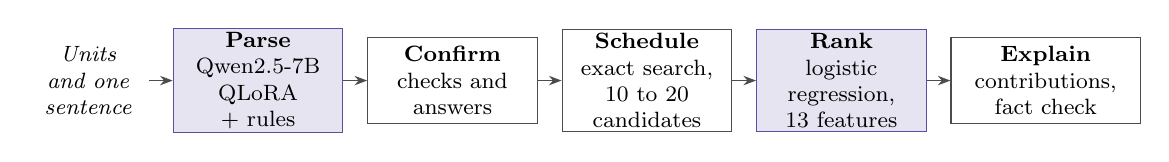
\begin{tikzpicture}[
	node distance=3mm and 3mm,
	box/.style={draw=black!70, align=center, font=\footnotesize,
		minimum height=11mm, text width=20.5mm, inner sep=1.5pt},
	ml/.style={box, fill=accent!15, draw=accent},
	code/.style={box, fill=white},
	io/.style={align=center, font=\footnotesize\itshape, text width=13mm},
	arr/.style={-{Stealth[length=1.6mm]}, black!70},
]
	\node[io] (in) {Units and one sentence};
	\node[ml, right=of in] (parse) {\textbf{Parse}\\Qwen2.5-7B\\QLoRA + rules};
	\node[code, right=of parse] (confirm) {\textbf{Confirm}\\checks and\\answers};
	\node[code, right=of confirm] (sched) {\textbf{Schedule}\\exact search,\\10 to 20 candidates};
	\node[ml, right=of sched] (rank) {\textbf{Rank}\\logistic regression,\\13 features};
	\node[code, right=of rank, text width=23mm] (explain) {\textbf{Explain}\\contributions,\\fact check};
	\draw[arr] (in) -- (parse);
	\draw[arr] (parse) -- (confirm);
	\draw[arr] (confirm) -- (sched);
	\draw[arr] (sched) -- (rank);
	\draw[arr] (rank) -- (explain);
\end{tikzpicture}

	\caption{The UniPlan pipeline. Shaded boxes are learned models; white boxes are code. The student confirms the parsed conditions before any timetable is built.}
	\label{fig:pipeline}
\end{figure}

\subsection{Parsing the Sentence}\label{sec:parse}

Rules split the sentence, a classifier labels each clause, and rules read the values; in an early four-sentence pilot, untrained Qwen models asked for all conditions at once dropped some and invented others.

We compared keyword rules, TF-IDF (term-frequency, inverse-document-frequency) character $n$-grams with logistic regression, Qwen2.5-7B with a detailed prompt and no training, and Qwen2.5-7B fine-tuned with QLoRA~\cite{dettmers2023qlora}. Training data came from a teacher-student loop: Qwen2.5-7B generated \sClauses{} labelled clauses in English, Chinese and mixed language, Claude graded \sGraded{} of them and wrote \sHardOne{} harder ones, and a second round added \sHardTwo{} Claude-written clauses aimed at round~1's two weakest labels, giving \sTrainTwo{} training clauses (\sClaudeTrainPct\% written by Claude) and \sValTwo{} validation clauses after rejected ones were removed. Fine-tuning took \loraMinutes{} minutes on one RTX~4090 Laptop GPU (Appendix~\ref{app:model}); the model was then quantised and served through Ollama. Round~2 replaced round~1 under a rule written before it was scored.

When unsure, the parser asks instead of guessing: when a second, cheaper classifier disagrees, when a clause could be hard or soft, or when a busy time has no day or hour. The student's answer overrides the model.

\subsection{Building Valid Timetables}\label{sec:schedule}

The scheduler enumerates every valid timetable exactly. It searches the activity groups with the fewest options first, removes every class that clashes with a chosen one, and backtracks as soon as a group has no class left; pairwise clashes are precomputed as bit sets and classes with the same times and places are searched once. Hard limits (clashes, unavailable times, full classes, walking time when set, day and hour limits, lunch) are checked on real dates, $G$, $D$ and $O$ are updated incrementally, and the non-dominated timetables are kept. Five units (\ttFive{} valid timetables) take \ttFiveSec{}~s on a Mac. If nothing is feasible, the scheduler names the clashing activities and offers the timetables that break the fewest limits, stating each; a clash is never allowed. We used no learning or approximation here: the search order affects only speed, and every valid timetable is still found. On 65 randomly generated problems, 40 with day, hour and lunch limits, it matched a slower reference search exactly in the number of timetables and their measures.

\subsection{Ranking the Candidates}\label{sec:rank}

Claude wrote \sPersonas{} student personas across ten situations (commuters, workers, parents, night owls and others), each a sentence with its intended conditions. For each persona the real scheduler produced candidates, and Qwen2.5-14B, playing the persona, chose between pairs shown as side-by-side tables. Each pair was asked in both orders and kept only if the answers agreed (\tKept{} of \tAsked{}, \tConsistent\%); when two timetables were almost equal on the persona's main concern, code decided by dominance or called a tie. Claude audited \tClaudeN{} of the teacher's labels without seeing its answers, agreed with \tClaudeAgree\%, and replaced the \sReplaced{} it disagreed with.

The deployed model was fitted to the first \rDeployPersonas{} training personas (\rDeployTeacher{} teacher pairs plus \rDeployCode{} dominance pairs, in which one timetable is no worse on any measure, labelled by code and not counted in Table~\ref{tab:data}), with the regularisation chosen by 5-fold cross-validation grouped by persona. A refit on all 120 training personas scored no better on the held-out personas (\rHeldTwo\% against \rHeldOne\%; \rHeldTeacherLR\% against \rHeldTeacherEq\% for equal weights on the pairs Qwen judged), so by a rule set beforehand it was not shipped. A random forest and a small neural network scored within one point in cross-validation, so we kept logistic regression, a ``glass-box'' model in the sense of the Week~11 lecture~\cite{engg2112_w11}: each score splits exactly into per-feature contributions, and the weights are a 4~KB file.

\subsection{Reasons, Evaluation and Environment}\label{sec:explain}

Each pick's reason is built from facts about its dated meetings and from the ranker's contributions, for example ``Vs option 2: 0.9 fewer days on campus a week and 1.8 fewer days a week with just one class; costs 2~h~53~min more waiting a week.''

Validation data and two development test sets, written in the coordinating Claude session, guided every design choice. The two final exams were written by fresh Claude agents that never saw the models, training data or model errors, committed after the models were frozen (Appendix~\ref{app:provenance}), and scored once. Intervals are 95\% bootstrap intervals resampling sentences or personas, paired when comparing methods. Training ran on a laptop RTX~4090 GPU (16~GB) and the web application on a Mac; every result has a seeded script and stored output. After the freeze the model weights, the ranker and the scheduler's search logic did not change, so the parsing and ranking scores are for the frozen models; we only added the closest-timetable fallback (scored separately in Section~\ref{sec:res-pipeline}) and changed wording and the web page.

\section{Results}\label{sec:findings}

\begin{figure}[h]
	\centering
	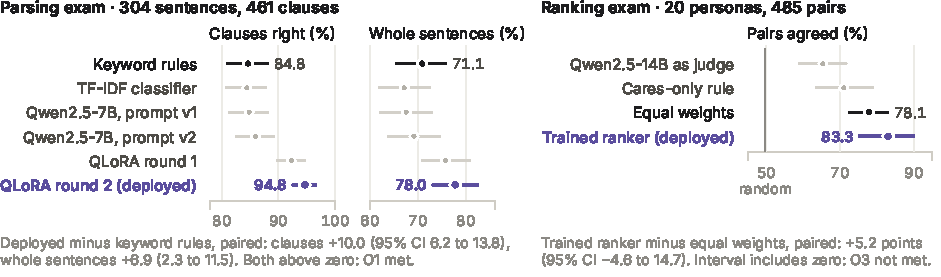
\includegraphics[width=\textwidth]{figures/fig_results.pdf}
	\caption{Both final exams (AI-written, scored once), each method with its 95\% bootstrap interval: (a,~b) parsing, (c) ranking, where the dashed line is chance. The deployed models are filled, the O1 and O3 baselines hollow black, the other methods hollow grey. Every value: Tables~\ref{tab:parse} and~\ref{tab:rank}.}
	\label{fig:results}
\end{figure}

\subsection{Parsing and Asking Back}\label{sec:res-parse}

Against the keyword-rule baseline of O1, the deployed model was \pDiffKeyC{} points better on clauses and \pDiffKeyS{} on whole sentences (paired 95\% CIs \pDiffKeyCLo{} to \pDiffKeyCHi{} and \pDiffKeySLo{} to \pDiffKeySHi; Figure~\ref{fig:results}). Fine-tuning made the difference: the same model untrained was no better than keyword rules, and training added \pDiffZeroC{} points on clauses (CI \pDiffZeroCLo{} to \pDiffZeroCHi) and \pDiffZeroS{} on whole sentences. Round~2 beat round~1 by \pDiffOneC{} points on clauses (CI \pDiffOneCLo{} to \pDiffOneCHi), but on whole sentences the difference is within noise. The offline fallback, TF-IDF with logistic regression, was chosen on validation data (\pLinVal\% of clauses against \pKeyVal\% for keywords; those clauses were mostly Chinese or mixed, the exam all English) but was no better than keyword rules on the exam; we did not switch afterwards. Splitting was exactly right for only \pSplit\% of sentences, the same for every classifier (a different split often still gives the same conditions), and most remaining sentence errors come from the rule-based steps.

The parser questioned \cAsked\% of clauses (\cAskedN, of which \cCovered{} were wrong), and \cSentWithQ\% of sentences got at least one question or offer. The questions covered \cCovered{} of the \cWrong{} wrong clauses, and for \cOption{} of them the correct reading was an option, so if students picked it clause accuracy would reach about \cProjected\% (a projection; no student answered).

\subsection{Ranking}\label{sec:res-rank}

The trained logistic regression agreed with the independent answers on \rLR\% of pairs and recovered \rLRTop{} of their top three (Table~\ref{tab:rank}); equal weights reached \rEq\% and \rEqTop. The paired difference is \rDiffEq{} points (95\% CI \rDiffEqLo{} to \rDiffEqHi), so the trained model is level with equal weights within the uncertainty: a rule that ignores what the student said does almost as well on this exam. Most of the deployed model's training pairs (\rDomShare\%) were dominance pairs, which push it towards the same choices as equal weights. The student terms helped against the teacher's labels (removing them cost \rAblInteraction{} points on 20 held-out personas) but are not shown to help on independent answers. Qwen2.5-14B judging pairs directly did worse (\rQwen\%), partly because it was asked each pair once and chose the first-shown timetable \rQwenFirst\% of the time, whereas teacher labels used both orders.

On the \rAgreePersonas{} personas answered twice, the two answerers agreed on \rAgree\% of pairs where both chose a side, similar to the human-human and human-LLM agreement of about 80\% reported in~\cite{zheng2023judge} and close to the model's score. Against the teacher's labels, accuracy was flat beyond 60 training personas, so more labels of the same kind are unlikely to help; whether better labels would is untested.

\subsection{Whole Pipeline and Reasons}\label{sec:res-pipeline}

On the parsing exam, \plExact\% of sentences (\plExactN{} of \sExamS) were parsed to exactly the intended conditions. Of the \plPlannable{} sentences whose parsed conditions allowed a timetable, \plViol{} (\plViolPct\%) received a recommendation that broke a stated condition. In half of them a clarifying question had already offered the fix, mostly hard-or-soft misreadings such as ``hates 8ams'', which the annotator treated as a limit and the parser as a preference; the rest came from splitting or number reading, such as ``no classes before 10 no classes after 4 no classes on friday'' written without commas. The first pick matched the one from the intended conditions in \plSameFirst\% of the \plSameFirstOf{} sentences where both had picks. Under the intended conditions, \plNoFit{} sentences (\plNoFitPct\%) had no timetable meeting every limit; the closest ones offered broke \plNoFitBreaks{} limits on average and never clashed (a post-freeze fallback).

All \exPicks{} template reasons passed the automatic fact check, as designed, and their main reason matched the ranker's largest contribution in \exMain\% of cases. The check's real use was on Qwen2.5-7B rewrites: only \exRewrite\% passed, and \exManualWrong{} of \exManualOf{} passed ones that Claude reviewed were still false, so the site shows templates only.

\subsection{Issues Faced}\label{sec:issue}

With the first ranking prompt, the teacher gave the same answer in both orders for only \tPilotFirst{} of \tPilotN{} pilot pairs. A side-by-side table, the main concern stated first and code-decided near-ties raised this to \tPilotAskedOK{} of the \tPilotAsked{} pairs still put to the 14B model (\tPilotFinal{} of \tPilotN{} with the code-decided ones). Students focused on waiting sometimes got more waiting, because code-labelled pairs favour fewer one-class days when waiting is equal.

\section{The End-to-End System}\label{sec:system}

UniPlan is a web application (\texttt{python3 main.py}). A student adds units and writes one sentence. The page writes what it read beside each clause and turns unsure clauses into two-option questions (Figure~\ref{fig:app}). Only after the student accepts or corrects these notes does the scheduler run. The student then sees three weekly grids with one-line reasons, can switch to all the distinct options kept, and can download a calendar file.

\begin{figure}[h]
	\centering
	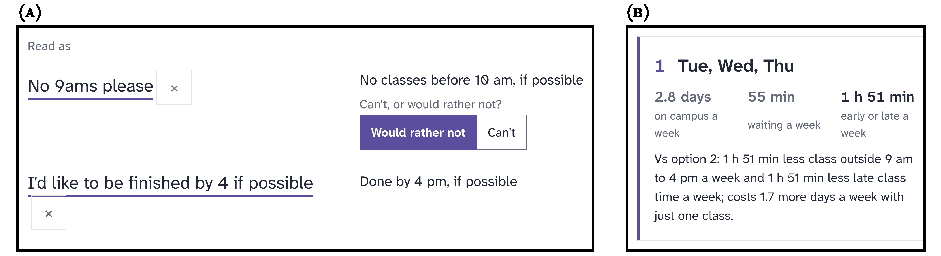
\includegraphics[width=\textwidth]{figures/fig_app.pdf}
	\caption{The web page with the deployed models on exam item e121 (AI-written). (a)~``No 9ams'' was read as a preference, so the page asks. (b)~After ``Can't'', the first of three picks with its reason.}
	\label{fig:app}
\end{figure}

Each AI output has a limited job. Parsed conditions are a draft that becomes binding only after the student confirms it; the ranking decides which timetables are shown first, never which exist; and the reasons come from the ranker's own contributions and are checked against the timetable. This follows the mixed-initiative pattern of the Week~7 lecture, where the AI points out missing constraints and the person decides~\cite{engg2112_w07}. The system also degrades gracefully: if the GPU server does not answer, it uses the model on the local machine and then, within 15~s, the TF-IDF classifier (\pRtwoC\% to \pLinC\% of clauses right on the exam), and asks the student to check each condition; if nothing fits, it names the clashing activities and offers the closest timetables with each broken limit stated.

\textbf{Deployment.} The run-time code uses only the Python standard library, and the fine-tuned model runs in Ollama on a single GPU. With the parser on one laptop GPU over the local network, a sentence for two to four units takes about \plMedianRec{}~s end to end, so one GPU server could serve many students, but enrolment opens for everyone at once and would need queueing; we did not load-test this. A real deployment would also need an official timetable feed or written permission from the university, seat numbers refreshed near enrolment day, and a pilot with real students (Section~\ref{sec:recs}).

\section{Stakeholders and Socio-Technical Issues at Scale}\label{sec:socio}

\textbf{Stakeholders.} Students gain time and a clearer view of their trade-offs; the timetabling office gains demand data but faces more concentrated demand; unit coordinators see class sizes shift; disability and carer services gain a way for students to state access needs in their own words. The likely adopter is the university or the student union rather than a paid app, since the run-time models are small and the value is faster enrolment.

\textbf{Demand would concentrate.} Thousands of students with similar wishes, such as no Friday classes, would be steered to the same classes, which would fill sooner; students who enrol last may lose most. A deployed version should show seat numbers and spread recommendations across equivalent classes.

\textbf{Accuracy may differ between students.} We tested only English written by an AI. Real students writing in a second language, or in Chinese or mixed language (most of the training clauses), may be misread more often, so accuracy should be measured per group of real students before launch, in line with the fairness principles of the Week~11 lecture~\cite{engg2112_w11}.

\textbf{The sentence is sensitive.} Students explain their week with a job, a disability or a family member who needs care. The Week~6 lecture warns about leakage and re-identification of personal data in AI systems~\cite{engg2112_w06}. UniPlan runs its models locally and needs no name or ID; a deployed service should discard sentences after use and never send them to a third-party model provider.

\textbf{People over-trust automated advice.} Users of decision aids tend to accept the first suggestion and miss its errors~\cite{parasuraman2010}, so a student may skim past a misread condition; margin notes and questions reduce but do not remove this risk.

\textbf{The model learned an AI's preferences.} The ranker was distilled~\cite{hinton2015distill} from Qwen2.5-14B playing students, so any bias in how these models imagine students, such as everyone wanting fewer days, is now in the weights; only real students can reveal it.

\textbf{Accountability.} A student who misses a class or a shift because of a recommendation bears the cost, so a service needs a named owner, a way to report errors, and a note that the official timetable rules.

\section{Recommendations, Transfer and Limitations}\label{sec:recs}

\textbf{Recommendations.} (1)~Before any release, run the pilot the proposal planned, with real students' own sentences and choices, accuracy reported per group, and a record of how often nothing fits (\plNoFitPct\% of exam sentences). (2)~Treat the learned ranker as unproven: in the pilot, compare it with equal weights on real choices and keep it only if it wins; on our exam it did not. (3)~Keep asking back: it covered most parsing errors at about \cPerSentence{} questions or offers per sentence. (4)~Improve splitting and number reading.

\textbf{Transfer to engineering scheduling.} The same structure fits wherever requirements are written in words and a schedule must satisfy hard constraints. A planner's note such as ``line 2 is down on Tuesday morning; keep changeovers low this week'' would become machine availability (hard) and changeover cost (soft); a solver with a time limit would replace exact enumeration, as a factory has too many schedules to list~\cite{pinedo2022}; and the ranker would learn from the plans planners actually chose, ordering feasible schedules by throughput, idle time and overtime. Misreads cost more there, so confirmation matters more. Text-to-optimisation work~\cite{ramamonjison2023nl4opt,ahmaditeshnizi2024optimus} could seed such a parser; none of this is tested.

\textbf{Limitations.}\label{sec:limits} No real student took part: all sentences, personas, labels and exams were AI-written, so the results show the method works on AI-written students, not that it helps real ones. The two exam annotators agreed on every parsing label, but they were the same model reading the same rules, and the exam writer removed \sExamDropped{} sentences the rules could not settle, so real sentences will be harder; Claude also wrote part of the training data and every persona, so the exams may share its style. The ranking exam has only \sRankExamPersonas{} personas, so its intervals are wide. The data covers one semester and \dUnits{} units, walking times are estimated, and none of the proposal's usability targets were measured.

\section{Conclusions}\label{sec:conc}

On AI-written exams UniPlan met O1 (\pRtwoC\% of clauses and \pRtwoS\% of sentences right, above keyword rules); met O2 for clashes, though \plViolPct\% of plannable sentences got a pick breaking a misread limit; and met O3 only in part (\rLR\%, level with equal weights). Whether real students would prefer these timetables is untested.


\clearpage
\bibliographystyle{IEEEtran}
\bibliography{refs}

\clearpage
\appendix
\addtocontents{toc}{\protect\setcounter{tocdepth}{1}}
\section{Use of Generative AI}\label{app:ai}

Generative AI was used in two different ways: as parts of the system, and as an assistant while building it. Both are listed here.

\subsection{AI Inside the System}

\begin{center}\small
\begin{tabular}{@{}>{\raggedright\arraybackslash}p{0.24\linewidth}>{\raggedright\arraybackslash}p{0.7\linewidth}@{}}
	\toprule
	Model & Role \\
	\midrule
	Qwen2.5-7B (fine-tuned) & Run-time clause classifier (Section~\ref{sec:parse}); served locally through Ollama. \\
	Qwen2.5-7B (untrained) & Generated the synthetic training clauses; zero-shot baseline; tried as a rewriter of reasons (switched off). \\
	Qwen2.5-14B & Teacher: labelled timetable pairs while playing each persona; direct-ranking baseline. \\
	Claude & In the coordinating session: wrote the two development test sets, \sHardAll{} hard training clauses and the \sPersonas{} personas, and graded and audited labels. Fresh agents that had seen no training data or models: wrote both final exams and answered the ranking exam. \\
	\bottomrule
\end{tabular}
\end{center}

\subsection{AI Used to Build the Project}

Claude Code (Anthropic) was used throughout development in the Claude desktop app. It wrote most of the code under the author's direction, ran the experiments, proposed and documented design changes, and drafted this report from the project's result files. OpenAI Codex helped draft and revise the proposal; that record is in the proposal's appendix. The author set the goals, made the design decisions recorded in Section~\ref{sec:change}, chose what to keep, and is responsible for the submitted work.

\subsection{Selected Prompts and Outputs}

The five exchanges below are from the main Claude Code conversation that coordinated the project (session \texttt{4ea07490}, stored locally by Claude Code). The author's messages are given in the original Chinese with an English translation; Claude's replies were in Chinese and are given as English translations, shortened, with [\ldots] marking omissions. Times are Sydney time (AEDT). Each is followed by what we changed and how the result was checked.

\newcommand{\who}[1]{\par\noindent\textbf{#1}\quad}
\newenvironment{exchange}[1]{\needspace{8\baselineskip}\subsubsection*{#1}\small}{\par}

\begin{exchange}{1.\ The system design (16 October 2026, 18:10 to 18:14)}
\who{Author:} 我直接用千问的开源模型就好了啊 / 我想的是我们有一个可视化的前端 然后只有判断逻辑接上大模型就好了 / 大模型只做语义分割 然后映射到我们设计好的条件里 然后由写好的程序来安排课表 然后再输出回大模型挑选 判断 \\
\textit{(``I'll just use Qwen's open-source model.'' / ``What I have in mind is a visual front end, with only the decision logic connected to the LLM.'' / ``The LLM only does semantic segmentation, then maps it to conditions we have designed; then a written program arranges the timetable; then it goes back to the LLM to pick and judge.'')}

\who{Claude:} ``[\ldots] There is one bottom line: deciding whether a timetable clashes must be done by the program, not by the LLM. The LLM will get times wrong, and recommending a timetable with a clash is a serious flaw. [\ldots] Understood, that is the flow. One correction on wording: in the report and the Q\&A say `semantic parsing' or `information extraction'. `Semantic segmentation' means per-pixel classification of images [\ldots] 1. LLM (parsing): turn the student's sentence into conditions in a fixed, pre-designed format [\ldots] 2. Program (scheduling): build every clash-free timetable from the hard conditions, then narrow them to 10 to 20 candidates [\ldots] 3. LLM (selection): read the student's words and the candidate summaries, pick the top 3 and write a reason for each. 4. Program (check): make sure the picks really are candidates; if not, ask again or fall back to a rule ranking. [\ldots] Show the parsed conditions to the student to confirm before scheduling.''

\who{What we changed:} We kept the split between learned parts and code and the confirmation step, and adopted the corrected terminology. We later fine-tuned the parser instead of only prompting it, and replaced the LLM in step 3 with a trained logistic ranker.
\who{How we checked:} On the final exam, Qwen2.5-14B judging pairs directly (asked once per pair) agreed with the answers on \rQwen\% of pairs, against \rLR\% for the trained ranker (Table~\ref{tab:rank}).
\end{exchange}

\begin{exchange}{2.\ Where machine learning belongs (16 October 2026, 18:58 to 19:00)}
\who{Author:} 回溯搜索是课程中有的吗 / 那我们就深化机器学习 然后我们可以先确定好算法是什么 \\
\textit{(``Is backtracking search covered in the unit?'' / ``Then let's go deeper on machine learning, and first settle which algorithms to use.'')}

\who{Claude:} ``It is not in the unit. I searched the slides for Weeks 1 to 11, lecture transcripts and tutorials [\ldots] That is fine [\ldots] scheduling is an ordinary engineering program whose job is to guarantee correct timetables; it is not the AI part. [\ldots] The core problem is classifying a student's clause into one of 9 condition types, a text classification problem. We solve the same task with a ladder of algorithms from simple to complex and compare them [\ldots] keyword rules; TF-IDF with logistic regression; [\ldots] Qwen without training; Qwen fine-tuned with LoRA. [\ldots] The test set is fixed before training and not changed afterwards.''

\who{What we changed:} We kept the ladder and the fixed test set, but did not build the naive Bayes and neural-network variants, and after a hand test dropped the 0.5B and 1.5B models and fine-tuned the 7B model instead.
\who{How we checked:} All remaining methods were scored on the same held-out exam (Table~\ref{tab:parse}).
\end{exchange}

\begin{exchange}{3.\ No human data, and the teacher-student loop (17 October 2026, 15:20 to 15:21)}
\who{Author:} 不需要组员了 基本都是我们做了 / 对 你出题 qwen来答 你判断对错 然后训练qwen \\
\textit{(``We don't need team members any more; we have done almost all of it.'' / ``Right: you write the questions, Qwen answers, you mark them, and then we train Qwen.'')}

\who{Claude:} ``[\ldots] The ranking check that team members were to answer will instead be answered by me (Claude) as a second annotator independent of Qwen. [\ldots] The report must say clearly that the test questions and check answers were produced by AI (Claude), not real students. [\ldots] It shows the system can parse and select accurately; it cannot show that real students will be satisfied. That goes into the limitations. [\ldots] This is the `teacher and student' approach: I am the teacher, Qwen is the student. [\ldots] The test set (the 142 sentences) is fixed before training; my training questions must not repeat it or paraphrase it. I will check the similarity of new questions to the test questions and delete those that are too close.''

\who{What we changed:} The synthetic-data statements in Sections~\ref{sec:data} and~\ref{sec:limits} follow this exchange. Because the first test set was later read while designing round~2, we added a second test set and the final exams.
\who{How we checked:} Similarity checks between training and test sentences, and exams written by agents that had not seen any training data (Appendix~\ref{app:provenance}).
\end{exchange}

\begin{exchange}{4.\ Guarding against over-fitting (17 October 2026, 19:56 to 20:22)}
\who{Author:} 我希望不要过拟合你能明白吗 / 对的 未来我们训练好后我也希望你能出很多新题 然后你来考我们训练好的模型 \\
\textit{(``I want to avoid over-fitting; do you understand?'' / ``Right. After the models are trained I also want you to write many new questions and examine our trained models.'')}

\who{Claude:} ``Understood. [\ldots] There are two kinds of over-fitting here: the model memorising the training questions, and us `tuning against the exam', which is subtler and more dangerous. [\ldots] The round-2 data was added after reading the round-1 errors on test v1, so v1 is no longer fair for round 2. I wrote v2 before starting round 2 [\ldots] I will fix the decision rule now, before the results [\ldots] Once every model is final, a brand-new `final exam', sat once, with nothing tuned afterwards. [\ldots] The questions are written by a fresh Claude subagent that receives only the labelling rules [\ldots] another independent subagent re-labels them [\ldots] the exam is committed and locked, with the time and a checksum, before any model is scored.''

\who{Author (20:22):} 不需要中英文混合 就是英文版就可以啊 \textit{(``No need for mixed Chinese and English; an English version is fine.'')}

\who{What we changed:} The plan proposed English, Chinese and mixed sentences; on the author's instruction the exam was English only, which Section~\ref{sec:socio} lists as a fairness limitation. The round-2 decision rule was committed before round 2 was scored.
\who{How we checked:} The commits, times and SHA-256 hashes in Appendix~\ref{app:provenance}.
\end{exchange}

\begin{exchange}{5.\ Restating and asking back (17 October 2026, 20:30)}
\who{Author:} 我还希望我们用自然语言描述需求之后这个模型还能给我们一些反馈 比如判断完复述一下判断结果 如果有不确定的还可以反问 而且也可以多嘴的问一些学生没提到 但是我们能做到的东西 你觉得是否能做到 \\
\textit{(``I'd also like the model to give feedback after a student describes their needs: restate what it understood, ask back when it is unsure, and even ask about things the student did not mention but we can handle. Do you think that can be done?'')}

\who{Claude:} ``It can, and it fits our structure well. [\ldots] 1. Restate: [\ldots] generated directly by the program from the parsed conditions, not written freely by the LLM, so it cannot misstate them. 2. Ask back when unsure, using three signals: the fine-tuned 7B and logistic regression disagree about a clause; the wording sits between `can't' and `would rather not'; a value is missing [\ldots] 3. Ask about things the student did not mention but we can do, such as a lunch break, in-person only, or days per week; at most 2, and easy to skip. [\ldots] The final exam can check whether the questions land where the model is really wrong.''

\who{What we changed:} Built as proposed; the restatement became margin notes beside each clause on the web page.
\who{How we checked:} On the exam the questions covered \cCoveredPct\% of wrong clauses (Section~\ref{sec:res-parse}).
\end{exchange}

\subsection{How AI Output Was Checked}

\begin{itemize}[leftmargin=*]
	\item \textbf{Code.} The repository has an automated test suite, including randomised tests that compare the fast scheduler with a slower reference search.
	\item \textbf{Models.} No model was scored on data written by its own family. The final exams were written by fresh Claude agents, frozen and hashed before scoring (Appendix~\ref{app:provenance}), and used once; the development test sets were written in the coordinating session and reused during development.
	\item \textbf{Labels.} Qwen's ranking labels were asked in both orders and audited by Claude without sight of Qwen's answers.
	\item \textbf{Reasons.} Every displayed reason passes a rule-based fact check against the timetable; the LLM rewriter was switched off when it failed this check too often.
	\item \textbf{This report.} Every number from our experiments is generated by a script from the result files in the repository, and each fact was traced to its source file before it was written. Three rounds of independent AI review, by sessions that had not seen the drafting, checked successive drafts against the marking rubric and recomputed about 60 numbers from the raw files.
\end{itemize}

\section{Data and Exam Provenance}\label{app:provenance}

The ranker (\texttt{llm/rank/model.json}) last changed at 18:02 on 17 October 2026 (commit \texttt{7ea2629}), before its exam was committed at 20:40 (\texttt{2eed03a}). The parser was frozen at git tag \texttt{exam-freeze} (commit \texttt{33ffb54}, 20:44 AEDT), before its exam was committed at 20:49 (\texttt{7e60a11}). Both exams were scored later that evening and not changed afterwards.

\begin{center}\small
\begin{tabular}{@{}ll@{}}
	\toprule
	File & SHA-256 (first 16 hex digits) \\
	\midrule
	\texttt{llm/parse/exam/exam.csv} & \texttt{195925d33cfb95fc} \\
	\texttt{llm/parse/exam/exam\_second\_annotator.csv} & \texttt{40895018c3d34595} \\
	\texttt{llm/rank/exam/personas.json} & \texttt{684178d7f5342a7e} \\
	\texttt{llm/rank/exam/questions.jsonl} & \texttt{dd160599ac5e755c} \\
	\texttt{llm/rank/exam/answers.jsonl} & \texttt{e3767ed281e849e8} \\
	\texttt{llm/rank/model.json} (deployed ranker) & \texttt{c4d2a264b6fd0450} \\
	\bottomrule
\end{tabular}
\end{center}

\section{Model Details}\label{app:model}

\textbf{Ranking features} (each a weekly average over the teaching weeks, standardised): days on campus; waiting between classes; minutes outside the student's comfortable hours, and separately the early and the late minutes; earliest start; latest finish; longest day on campus; most class hours in a day; Friday free; building changes; days with only one class; share of online classes.

\textbf{Parser fine-tuning} (round~2): the Qwen2.5-7B Instruct model in 4-bit NF4 precision with LoRA adapters of rank \loraRank{} and $\alpha=\loraAlpha$, learning rate \loraLR, \loraEpochs{} epochs, best validation epoch \loraBest, \loraMinutes{} minutes on one RTX~4090 Laptop GPU (round~1: \loraMinutesOne{} minutes).

\section{Repository Guide}\label{app:repo}

Code: \repo

Every number and table in this report is regenerated from the result files by \path{report/scripts/make_numbers.py}. The repository's README lists the final models and how to run and reproduce everything.
\begin{itemize}[leftmargin=*]
	\item Deployed ranker: \path{llm/rank/model.json}.
	\item Deployed parser: the Ollama model \path{uniplan-parse-7b-r2}, trained by \path{llm/parse/windows/train_lora.py} (the 7B weights are too large for the repository).
	\item Offline fallback parser: \path{llm/parse/output/linear_model.json}.
	\item Scheduler: \texttt{uniplan/schedule.py}; web application: \texttt{main.py}.
	\item Every other model in the comparisons, with its training script and outputs: \path{llm/parse/} and \path{llm/rank/}.
\end{itemize}

\section{Contributions}\label{app:contrib}

The project was completed by one member, Han Dongrui, with the generative AI assistance described in Appendix~\ref{app:ai}. The report uses the conventional authorial ``we''.


\end{document}
